\documentclass[twoside]{article}

\usepackage{lipsum} % Package to generate dummy text throughout this template

\usepackage{float}
\usepackage{amssymb}

\usepackage[sc]{mathpazo} % Use the Palatino font
\usepackage[T1]{fontenc} % Use 8-bit encoding that has 256 glyphs
\linespread{1.05} % Line spacing - Palatino needs more space between lines
\usepackage{microtype} % Slightly tweak font spacing for aesthetics

\usepackage[hmarginratio=1:1,top=32mm,columnsep=20pt]{geometry} % Document margins
\usepackage{multicol} % Used for the two-column layout of the document
\usepackage[hang, small,labelfont=bf,up,textfont=it,up]{caption} % Custom captions under/above floats in tables or figures
\usepackage{booktabs} % Horizontal rules in tables
\usepackage{float} % Required for tables and figures in the multi-column environment - they need to be placed in specific locations with the [H] (e.g. \begin{table}[H])
\usepackage{hyperref} % For hyperlinks in the PDF

\usepackage{lettrine} % The lettrine is the first enlarged letter at the beginning of the text
\usepackage{paralist} % Used for the compactitem environment which makes bullet points with less space between them

\usepackage{graphicx}
\usepackage{listings}
\usepackage{amsmath}
\usepackage{mathtools}

\usepackage[dvipsnames]{xcolor}

\usepackage{abstract} % Allows abstract customization
\renewcommand{\abstractnamefont}{\normalfont\bfseries} % Set the "Abstract" text to bold
\renewcommand{\abstracttextfont}{\normalfont\small\itshape} % Set the abstract itself to small italic text
\usepackage{color}
\lstset{language=Haskell,
                basicstyle=\ttfamily,
                keywordstyle=\color{blue}\ttfamily,
                stringstyle=\color{red}\ttfamily,
                commentstyle=\color{ForestGreen}\ttfamily,
                morecomment=[l][\color{magenta}]{\#}
}

\usepackage{titlesec} % Allows customization of titles
\renewcommand\thesection{\Roman{section}} % Roman numerals for the sections
\renewcommand\thesubsection{\Roman{subsection}} % Roman numerals for subsections
\titleformat{\section}[block]{\large\scshape\centering}{\thesection.}{1em}{} % Change the look of the section titles
\titleformat{\subsection}[block]{\large}{\thesubsection.}{1em}{} % Change the look of the section titles

\usepackage{fancyhdr}
\pagestyle{fancy}
\lhead{CS166: Data Structures}
\rhead{June 2016}

%----------------------------------------------------------------------------------------
%	TITLE SECTION
%----------------------------------------------------------------------------------------

\title{\vspace{-15mm}Abstract Dynamic Prefix Codes \\ \vspace{0.5em} \Large An Application of Splay Trees to Image Compression} % Article title

\author{
 % Your name
\normalsize Mitchell Douglass \,\,\,\,\,\, Ryan Hermstein \,\,\,\,\,\, Colin Kincaid \\\\
Stanford University
\vspace{-5mm}
}
\date{}

%----------------------------------------------------------------------------------------

\begin{document}

\maketitle % Insert title

\thispagestyle{fancy} % All pages have headers and footers

\begin{abstract}

\noindent We do explore an abstract framework for data encoding in which any binary tree strategy may serve as the basis of a prefix code. We demonstrate how this framework applies to popular prefix codes, such as the Huffman code, which provides optimally-concise, static prefix codes. We explore how dynamic binary tree strategies can produce dynamic prefix codes that preserve many of the same properties while yielding significantly more concise encodings for data with certain properties, which we discuss. In particular, we implement a prefix code using a modified version of the splay tree, and we perform various experiments comparing its performance to that of simpler codes. We find that, by combining our splay code with a transformation defined by a plane-filling curve, we achieve reasonable lossless compression of image data.

\end{abstract}

\begin{multicols}{2} % Two-column layout throughout the main article text

\section{Introduction}

In the realm of modern computing challenges, one of the richest topics for exploration is data encoding. Encoding refers to the transformation of a set of data into a different form, from which the original can be recovered through a corresponding decoding process. The applications of data encoding are numerous and include such tasks as password encryption, network communication, and the focus of this paper: data compression.

Uncompressed files use well-delineated, full bytes to represent their characters, but data encoding allows us to keep track of the same information in less space. One technique by which we can reduce the space a file takes up is bit encoding; that is, rather than work with entire bytes at a time, we represent characters with variable-length bit sequences. From these sequences, we can recover characters with complete fidelity when encoding. At the same time, because we are not bound to using eight bits per character--and can actually use fewer than eight in many cases--we are often able to store entire files using less space than their original versions.

A specific encoding scheme useful in data compression is the prefix code. In a prefix code system, no encoding can be the prefix of any other distinct encoding. As a result, prefix code encodings are self-delineating when read bit-by-bit: We need neither knowledge of the number of bits used per character (as is the case in an uncompressed eight-bit representation) nor a demarcator telling us where one code ends and the next begins. 

Perhaps the most well-known prefix code algorithm is Huffman coding. The Huffman encoding scheme creates a weight-balanced tree in which characters are weighted based on their frequencies across a static data set. More frequent characters appear close to the top of the tree, while less frequent characters appear closer to the bottom. Each parent-child link in the tree corresponds to a bit, and traversal in the tree encodes a character based on which edges were followed in order to find it. Furthermore, characters are only stored in the leaves of Huffman trees, so the prefix property of the encodings generated this way is guaranteed.

Huffman encoding is optimal for static data sets, but numerous innovations have improved upon the algorithm by making the encoding tree more adaptive [2]. This paper will explore the application of splay trees as a tool to space-efficiently encode dynamic data sets. We specifically examine the problem of compressing image files, experimenting with an encoding pipeline in which images are first transformed using plane-filling curves in order to maximize the benefits of splay tree encoding.

%\begin{itemize} 
%\item Data encoding (Colin)
%\item Prefix Codes (Colin)
%\item Huffman, it's statically optimal (Colin)
%\end{itemize}

\vspace{-0.5em}
\section{Abstract Prefix Code Model}

%\begin{itemize}
%\item Any static prefix code corresponds to a static binary tree. (Mitchell)
%\item Examples of good and bad static prefix codes. (Mitchell)
%\item Dynamic prefix codes. (Mitchell)
%\item Formal description of framework, giving required conditions for a dynamic prefix code to work. (Mitchell)
%\end{itemize}

In this section, we aim to describe an abstract framework for prefix codes based on binary tree strategies. Our framework will apply to the static prefix codes, such as the Huffman code, but will also expand the realm of possibile prefix codes. Specifically, we will see how this framework allows for construction of dynamic prefix codes when we apply our framework with dynamic binary trees.

First, we define what is meant by $static$ and $dynamic$ prefix codes in the context of our model. A code defines an invertible mapping from \textbf{message words}, the alphabet from which messages are constructed, to \textbf{code words}, the alphabet of encoded messages. We denote the set of message words by $\mathcal{M}$, and we denote the set of code words by $\mathcal{C}$. A code is allowed to depend on a context of zero or more message words, so long as the code remains invertible given a fixed context. Formally:

\vspace{0.5em}
\noindent \textbf{Definition.} A \textbf{code} is a a pair of mappings
\begin{align*}
&E: \mathcal{M}^* \times \mathcal{M} \to \mathcal{C}\\
&D: \mathcal{M}^* \times \mathcal{C} \to \mathcal{M} \cup \{\bot\}
\end{align*}
such that for all message words $m \in \mathcal{M}$ and contexts $\alpha \in \mathcal{M}^*$, we have $D(\alpha, E(\alpha, m)) = m$ and $D(\alpha, x) = \bot$ if $x$ does not encode any message word under the context $\alpha$. A code that does not depend on its context is called a \linebreak \textbf{static code}, while a code that does depend on its context is called a \textbf{dynamic code}.

\vspace{0.5em}
This definition of a code suggests a natural method for encoding and decoding messages. Notice that messages correspond to elements of $\mathcal{M}^*$ (which includes the empty sequence $\epsilon$). Suppose $m = m_1\cdots m_n \in \mathcal{M}^*$ is a message to be encoded. Let the encoded message be $c = c_1 \cdots c_n$, where $c_i = E(m_1\cdots m_{i-1}, m_i)$. For this encoding to be useful, we require that it be possible to recover the message $m$ from $c$, and indeed it is possible. Note that $m_1 = D(\epsilon, c_1)$, and given $m_1, \dots, m_{i-1}$ we can decode $m_i$ as $D(m_1 \cdots m_{i-1}, c_i)$. This encode/decode strategy has a clear procedural analogy: encoding and decoding routines operate word by word, applying the appropriate mapping at each step, using the sequence of previously seen (or computed) message words as context. As we will soon see, the "context" of the encoding and decoding procedures will not usually be an explicit list of message words, but rather algorithmic state which is a direct function of these message words. As a final note, the name "static code" comes from the fact that a message encoded as above using a static code is such that a particular message word $m_0 \in \mathcal{M}$ is always encoded by the same code word $E(\cdot, m_0)$, whereas the same is not true of dynamic codes.

When implementing codes in a computer system, we require that message words and code words themselves be encoded in bits; i.e. using the alphabet $\{0, 1\}$. This introduces the following dilemma: How do our encoding and decoding procedures know where the message and code word boundaries lie? For message words, the dilemma is easily resolved; we will work with codes in which each message word is a sequence of eight bits, also known as a byte. This is a reasonable restriction to impose, since many forms of data (ASCII characters, pixel luminance, etc.) are logically represented by byte sequences. However, for reasons which will soon be clear, we do not wish to fix the length of code words. Instead, consider the following property as a resolution to this dilemma:

\vspace{0.5em}
\textbf{Definition. } A \textbf{prefix code} is a code $(E, D)$ such that, for all contexts $\alpha \in \mathcal{M}^*$ and distinct message words $x, y \in \mathcal{M}$, we have that the code word $E(\alpha, x)$ is not a prefix for $E(\alpha, y)$, considered as bitstrings. We say that a prefix code is \textbf{prefix-free}.

\vspace{0.5em}
A prefix code resolves the above dilemma of code word length. Suppose the context of previously decoded message words is $\alpha \in \mathcal{M}^*$. To determine the next code word, a decoder simply reads subsequent bits, one at a time, from the encoded message, constructing a candidate code word $c$. So long as $D(\alpha, c) = \bot$, it is clear that more bits must be read to construct the next code word. However, once it is the case that $D(\alpha, c) \in \mathcal{M}$, it is clear that the next code word has been read in full, since now $c$ is a valid encoding of the message word $D(\alpha, c)$ and therefore, by the prefix-free property, no code word extending $c$ can be a valid encoding of a message word given $\alpha$ as context.

With the above machinery in place, we can now give a full characterization of static prefix codes, as follows:

\vspace{0.5em}
\noindent \textbf{Proposition 1. } Static prefix codes are in direct correspondence with the set of binary trees with $|\mathcal{M}|$ leaves, where leaves are labeled uniquely by message words $\mathcal{M}$.

\vspace{0.5em}
\textit{Proof. } Let $B$ be a binary tree with $|\mathcal{M}|$ leaves, labeled uniquely by $\mathcal{M}$. Label edges in $B$ by $0$ if they follow into a left subtree and $1$ if they follow into a right subtree. Define a code $(E, D)$ such that $E(\cdot, m)$ is equal to the bitstring of edge labels along the path from the root of $B$ to the node labeled by $m$, and $D(\cdot, c)$ is equal to the label of the leaf attained by following a path defined by the bits of $c$ corresponding to the edge labels of $B$. Since two paths from the root of $B$ to distinct leaf nodes must diverge at the lowest common ancestor of these leaves, and since the labels of the outward edges of this ancestor are different, we see that the encoding function is injective, and by extension that the decoding function succeeds in inverting it. The resulting code must be a prefix code, since otherwise decoding a code word $cx$ which extends another code word $c$ would imply that the leaf labeled by $D(\cdot, c)$ is an ancestor of the leaf labeled by $D(\cdot, cx)$. It is a static code because $B$ is fixed.

Now suppose $(E, D)$ is a static prefix code. Consider, for each message word $m \in \mathcal{M}$, inserting the bitstring $E(\cdot, m)$ into a trie (with alphabet $\{0, 1\}$). Label trie nodes corresponding to completion of $E(\cdot, m)$ with $m$. Because $(E, D)$ is a prefix code, the nodes labeled in this way must be leaves in the trie. Associate $0$ edges with left subtrees and $1$ edges with right subtrees to produce the required binary tree. \nolinebreak $\blacksquare$

\vspace{0.5em}
In light of Proposition 1, we can easily relate various encoding schemes to binary tree structures. For instance, notice that the identity encoding $E(\cdot, m) = m$, $D(\cdot, c) = c$ is given by a perfectly balanced binary search tree on the message words $\mathcal{M}$ (while we don't require an ordering on $\mathcal{M}$ in general, here we order bytes by integer value). If we do this, we end up with a tree whose structure assigns each message word a codeword exactly matching the bit pattern of the message word byte, from most significant bit to least significant bit. We can build a static prefix code which simply permutes the message word bytes by building balanced binary search tree as before, but choosing a non-standard ordering on $\mathcal{M}$ in order to produce the desired permutation. Finally, we can construct codes that are not concerned with efficient encodings, such as the "unary" code below in which characters are represented by runs of $1$'s separated by $0$s.

\begin{center}
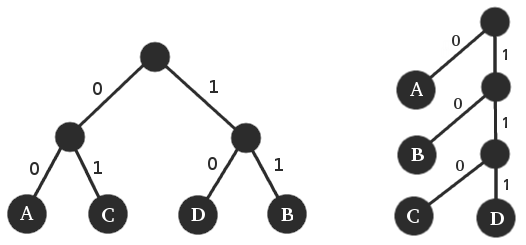
\includegraphics[scale=0.35]{staticid_unary}
\textbf{Figure 1:} A permutation and unary code.
\end{center}

As a slightly more nuanced example, consider the case of determining a binary encoding for a set of message words $\Sigma$ of arbitrary size. As we did with our set $\mathcal{M}$ of 256 message words, we can construct a prefix code based on a balanced tree with the words of $\Sigma$ as leaf nodes. Without having to check the details, by Proposition 1, this produces a valid, static prefix code.

Before we proceed to provide a formal description of our general framework, we touch on two more strategies that we would like our framework to address.

First, the Huffman code introduces a new consideration. A Huffman encoder fits into the above framework in that its main operational phase involves encoding message words into code words using a fixed binary tree (i.e., a static prefix code). However, this static prefix code is dependent on the particular message being encoded. Specifically, a Huffman coder builds its binary tree based on a table of message word frequencies. If these frequencies are not common knowledge, this table must be included in an encoded message so that any decoder can construct the same binary tree in order to decode the static code. Notice that such a "message digest" does not grow with the size of the message (assuming the transdichotomous model, in which the length of a message fits into a constant number of bytes). In fact, the Huffman code, on a constant-sized alphabet, requires a constant number of bytes to encode this message digest. Therefore, our framework will allow for strategies that require such message digests.

Finally, and most importantly, we would like our codes to allow for dynamic prefix codes. Recall that a code $(E, D)$ is dynamic if these mappings depend on the context of message words that they are provided. In theory, dynamic prefix codes are in correspondence with mappings from $\mathcal{M}^*$ to the set of binary trees described in Proposition 1. The justification of this follows in the same spirit as that for the proposition; in this case, we may use a different binary tree for each context. In other words, a dynamic code $(E, D)$ can be thought of as implementing a different static prefix code $(E(\alpha, \cdot), D(\alpha, \cdot))$ for each possible context $\alpha$. For our purposes, it will suffice to consider dynamic codes based on binary tree strategies. Suppose $B$ is a dynamic binary tree such that, given a path from its root to a leaf node, $B$ may perform structural modifications to its node structure, in number proportional to the length of the root-leaf path. Of course, we require that $B$ maintain $|\mathcal{M}|$ leaf nodes labeled by the message words of our code. If this is the case, then the dynamic binary strategy of $B$ provides a dynamic prefix code $(E, D)$. First, choose an an initial structure $B_0$ for the dynamic binary tree $B$. The code static prefix code $(E(\epsilon, \cdot), D(\epsilon, \cdot))$ is given by $B_0$. For a sequence $m_1 \cdots m_i \in \mathcal{M}^*$, the static prefix code $(E(m_1 \cdots m_i, \cdot), D(m_1 \cdots, m_i, \cdot))$ is given by the structure of $B$ after a sequence of restructuring procedures given by root-leaf paths to $m_1$, then $m_2$, and so on until $m_i$, in that order. With access to the $m_1, \dots, m_i$ of the message, an encoder need only determine the root-leaf paths in order to perform the restructuring procedures. A decoder may also perform the restructuring procedures since, before decoding $c_{i+1}$, it is given the root-leaf paths for $m_1, \dots, m_i$ in the code words $c_1, \dots, c_i$.

In summary, we have developed a general framework for constructing prefix codes using binary tree strategies:

\vspace{0.5em}
\noindent \textbf{Framework. } Suppose we have access to the following:

\begin{enumerate}
\item A \textbf{Digest Function}, which produces message digests of size $O(|\mathcal{M}|)$, given a message in $\mathcal{M}^*$.
\item An \textbf{Initialization Function}, which produces an initial binary tree structure $B_0$, given a message digest.
\item A \textbf{Dynamic Tree Strategy}, which performs $O(x)$ restructuring operations of a binary tree $B$, given a path of length $x$ from the root of $B$ to a leaf node.
\end{enumerate}

Then we can construct a corresponding dynamic prefix code from these components, as detailed by this section. Of course, the code need not be strictly dynamic. For instance, the Huffman code fits into this framework by implementing parts 1 and 2 above, letting the restructuring component of 3 be a no-op.

In this section, we have not explored the possible dynamic tree strategies that can be applied in this framework. For the remainder of this paper, we explore exactly this.

\section{Splay Trees}

%\begin{itemize}
%\item "We intend to use splay trees in a dynamic prefix code". (Mitchell)
%\item Brief and informal description of splay tree operation. (Mitchell)
%\item Mention of splay tree amortized $O(\log n)$ efficiency (implies that a prefix code based on splay tree cannot blow up file data by an arbitrary factor). (Mitchell)
%\item Mention of the Working Set Theorem. Aparently the proof is pretty tough, though we might try it. (Mitchell)
%\end{itemize}

Splay trees are a dynamic binary search tree data structure originally introduced in a landmark paper by Sleator and Tarjan [4]. Splay trees operate much the same way as balanced binary search trees, except that splay trees perform structural adjustments, called tree rotations, along the path of any root-node search path. These adjustments are designed such that tree nodes along a root-node search path are benefited in terms of their proximity to the root node.

We do not present the complete and formal rules of splay tree operation, as these can be found in the aforementioned paper. Instead, we wish to investigate the interesting properties that splay trees gain as a result of their dynamic strategy. In particular, we will study the implications of known runtime characteristics of splay trees on the performance of a splay tree used in the frame work of section II. Although necessary modifications to the original splay tree will be given in section IV, the results studied here will still apply. We will say "splay tree prefix code" or simply "splay code" to refer to a dynamic prefix code, in the framework of section II, built on top of the dynamic binary tree strategy of splay trees.

First, we mention a useful framework for proving results about the runtime of splay trees. We then state a number of well-known results about the runtime of splay trees, which can be shown given this framework. Since these results are laid out in detail in [4], we do not give formal proofs here.

\vspace{0.5em}
\noindent \textbf{Theorem 1. } Let $x_1, \dots, x_n$ be the keys stored in a splay tree, and assign to each key $x_i$ a positive weight $w_i$. Let $W = \sum_i w_i$. Let $W(x_i)$ be the sum of weights of all keys in the subtree rooted by $x_i$. Finally, define a potential function by $\Phi = \sum_i w(x_i)$. Then the amortized cost of accessing a node with key $x_i$ is given by
\[
1 + 3\log(W/w_i)
\]

This useful fact allows us to discover a handful of interesting theorems about the runtime of splay tree accesses.

\vspace{0.5em}
\noindent \textbf{Theorem 2 (Balance Theorem).} The total amortized cost of performing $m$ accesses is $O(m \log n + n \log n)$.

\vspace{0.5em}
This result follows from choosing weights $w_1 = \dots = w_n = 1$. Note that if $m = \Omega(n)$, then this gives a total amortized access time of $O(m \log n)$. This has an important implication for any data encoding algorithm based on a splay tree. Note that a message of $m$ words from a message word set of size $n$ can be encoded by a fixed-width code in $m \log n$ bits. A prefix code algorithm as outlined in the framework of section II will output a number of bits proportional to the runtime of the encoding algorithm. Therefore, this Balance Theorem shows that a message encoded by a prefix code built on the splay tree cannot be blown up by more than an absolute constant (specifically, the constant associated with the $O(m\log n)$ of the theorem's result). Consequently, The Balance Theorem also gives us an upper bound on the runtime of a prefix encoder based on a splay tree.

The following result draws an interesting link to Huffman encoding.

\vspace{0.5em}
\noindent \textbf{Theorem 3 (Static Optimality Theorem).} Suppose a splay tree storing keys $x_1, \dots, x_i$ undergoes a sequence of $m$ accesses in which each key $x_i$ is accessed at least once. Let $f(x_i)$ denote the number of accesses of key $x_i$. Then the total amortized runtime is 
\[
O \big ( m + \sum_i f(x_i) \log \frac{m}{f(x_i)} \big )
\]

\vspace{0.5em}
The result is achieved by choosing weights $w_i = f(x_i)/m$. The sum in this expression is equal to $m$ times a quantity known as the Shannon Entropy of a message, discussed in more depth at the start of section VI. In short, the Shannon Entropy describes the theoretical minimum number of bits required to encode a message word from a the set of $n$ message words, given that the only known property of a message is its message word frequencies. The Huffman code is designed explicitly to achieve this minimum number of bits specified by the Shannon Entropy. What the Static Optimality Theorem tells us is that a data encoding scheme based on splay trees is guaranteed, in the worst case, to produce encodings of size approaching those of a Huffman code, to within a fixed constant factor.

The Balance Theorem told us that prefix codes built on splay trees will not produce arbitrarily bad encodings. The latter theorem shows that these splay codes will produce codes that are roughly as good as the Huffman code. The following result motivates why we believe splay codes can dramatically outperform the Huffman code.

\vspace{0.5em}
\noindent \textbf{Theorem 4 (Working Set Theorem). } Suppose a splay tree storing keys $x_1, \dots, x_n$ undergoes a sequence of $m = \Omega(n \log n)$ successful access queries, the amortized per-operation cost of each access is $O(1 + \log t(x_i))$, where $t(x_i)$ is defined to be the number of elements accessed since the last access of $x_i$.

This theorem has profound implications on the performance. Given a small message word set of $n = 256$ bytes, it is not unreasonable to assume that the encoding of any interesting file will require $\Omega (n \log n)$ message word encodings. Now suppose that a stream of bytes being encoded by a splay prefix encoder enters a "working set" in which a long sequence of bytes exhibits only 16 unique values. In this case, the Working Set Theorem tells us that the bytes of this extended sequence will be encoded with a maximum of $\log 16 = 4$ bits, a compression factor of 2! This property follows from the fact that splay trees bring recently accessed nodes up to the top of the tree, and therefore essentially produce a balanced binary tree of recently accessed items at the top of the tree, which can be oblivious to nodes residing underneath if they are not accessed.

In this section, we have surveyed well-known runtime results of splay trees and related them to implied compression performance of a dynamic prefix code based on splay trees. But we have not justified the fact that splay trees are a valid binary tree strategy for use in our framework, since after all the standard tree node operations cause nodes to become the root of the splay tree and therefore an unmodified splay tree strategy cannot maintain a fixed set of leaf nodes. In the next section, we show the required modifications to incorporate a splay tree strategy into our framework.

\section{Splay Tree Prefix Code}

%\begin{itemize}
%\item Modifications to the Splay tree. Some modifications are necesary for prefix codes, while others simplify the algorithm. (Ryan)
%\item A discussion of why the above changes do not change the desireable properties of splay trees. (Maybe we can do some analysis on this, since the splay is different: not splay-to-root). (Ryan, +Mitchell on analysis)
%\end{itemize}

We will now examine how splay trees fit into the framework developed in section II. Splay trees are a type of dynamic binary tree, so we know that we can apply abstract prefix code framework and use them for data compression. As we have previously described, splay trees are statically optimal. Static optimality is concerned with the total number of nodes touched during a lookup. This directly relates to the total number of bits written to a compressed file using the previously described framework. Thus, it is apparent that splay trees should have some value in this field.

The actual splay tree compression algorithm described in [2] uses a modified splay tree. This modified splay tree has several key differences from the original splay tree described in [4]. Note that in our framework, character nodes must be leaf nodes. This means that splaying nodes up to the root as done in the original splaying algorithm will not work. However, the biggest difference in this problem compared to other applications of traditional splay trees is the fact that no data are stored in internal nodes. Traditional splaying would make these nodes with data no longer be leaves by shuffling child nodes around, invalidating the data structure and causing problems. We avoid this roadblock using a variant on splaying called semi-splaying, which does not modify the children of the target nodes. Furthermore, semi-splaying has been shown to achieve the same theoretical efficiency bounds as splaying, within a constant factor [2]. 

We will now describe semi-splaying in more detail. The only difference from Sleator and Tarjan's original splaying algorithm [4] is in the zig-zig case. After rotating the parent with the grandparent, the original node is not rotated with the parent. Instead, splaying continues from the parent instead of the original node. Consequently, the original node being accessed is not splayed up to the root. The effect of semi-splaying is that it reduces the depth of every node on the access path to at most about half of its previous value [2]. This means that after at most $log_2n$ (where $n = |\Sigma|$) repetitions of accessing a particular character, that character's node will be the child of the root and have a one-bit code. This also means that semi-splaying does not adapt as quickly to changes. Rather, semi-splaying shines when the access pattern is more stable and there are long strings of the same character. Furthermore, semi-splaying does not penalize other nodes as much when a node is accessed. This is because the accessed node does not move all the way to the root immediately, so the tree retains more of its original structure per semi-splay. Thus, infrequent characters in a region of mainly one specific character will not hurt this data structure. 

The actual splaying used by the data compression algorithm is a variation of semi-splaying optimized for a prefix code tree. The alterations from standard semi-splaying do not affect the functionality of the overall algorithm; they merely simplify the splay operation for this particular scenario. Unoptimized semi-splaying would also work in this algorithm.

We will now describe these variations on semi-splaying. The first variation is an operation called twisting. Twisting the tree involves modifying each node on the access path. Any nodes that are right children are exchanged with their siblings. This eliminates the need for a zig-zag case, which is the most complicated case in semi-splaying.

We will now show that this twisting before semi-splaying does not affect the performance bounds that have been proven for semi-splaying. 

\textit{Proof:} Twisting the tree before semi-splaying does not change the performance bounds. First, consider the potential function used for the amortized analysis of splaying. We will define the size $s(x)$ of a node $x$ to be the total weight of all items in the subtree rooted at $x$. The rank $r(x)$ is $log(s(x))$. The potential function is the sum of the ranks of all the nodes in the tree. Note in Figure 1 (from [2]) that every node in the tree has the same nodes in its subtrees--though perhaps in a different configuration--before and after twisting. Thus, potential function is unaffected by twisting. Furthermore, twisting takes $O(1)$ time, so it does not incur any extra costs compared to splaying when traversing the tree. Thus, twisting the tree before semi-splaying does not change the performance bounds that have already been established for semi-splaying. $\blacksquare$

The second variation arises from the fact that internal nodes carry no information. Exchanging two internal nodes is unnecessary, so we can further simplify the semi-splaying done for this data compression algorithm. Instead of semi-splaying, only two links need to be exchanged: the grandparent's child link with the target node's parent link. This operation, shown in Figure 2 (from [2]) is known as a semi-rotation. There is no need to twist the tree before applying semi-rotations. Rather, semi-rotations have the same effect as twisting the tree before semi-splaying, as long as internal nodes are considered anonymous. 

Semi-rotations will serve as the foundation for the splaying employed by this data compression algorithm. Now that we have described the splaying, we can describe the algorithm itself. We will use a bottom-up approach. We store the following data in each node:

\begin{lstlisting}[language=C++]
struct treeNode {
    unsigned short ch;
    struct treeNode* parent;
    struct treeNode* left;
    struct treeNode* right;
}
\end{lstlisting}

The character field of each node is an unsigned short because we need an extra character for a stand-in end-of-file character (PSEUDO\_EOF). We also have a HashMap mapping each possible character to the corresponding leaf node. This way, we can easily start the walk up the tree. Now that we have described the data we have at hand, we will describe the data compression algorithm, beginning with the encoding step.  

At the start of the encoding step, the entire tree is built as a balanced, full tree. It has 257 leaf nodes, one for each character and one for PSEUDO\_EOF. This initial setup does not matter as long as the encoder and decoder agree on the same starting tree format. The input is read one character at a time and the following is done for each character:
\begin{itemize}
\item Use the HashMap to get the leaf node corresponding to that character.
\item Walk up the tree using the parent pointers, pushing bits onto a stack accordingly (a 0 if a left link was taken and a 1 if a right link was taken) until the root is reached.
\item Pop each bit from the stack and write each bit to the compressed file. This writes them in the proper order for traversing the tree from the root down to the character's node.
\item Splay the tree starting at the leaf node for the character. This involves doing semi-rotations for each pair of nodes on the access path.
\end{itemize}

Lastly, PSEUDO\_EOF is written the output. This is the end of the encoding step.

Now we will describe the decoding process. After building the initial tree like in the encoding step, the current node pointer is set to the root. Bits are read from the input one at a time, and the tree is traversed accordingly. A left link is taken if a 0 bit is read and a right link is taken when a 1 is read. When a leaf node is reached, the node's character is sent to the output and the tree is splayed from that node. The splaying operation is exactly the same as in the encoding step with the semi-rotations in pairs. This process repeats until the PSEUDO\_EOF character is reached.

It turns out that this type of data compression has several advantages. Aside from the simple gains over other compression algorithms such as speed and simplicity, data compression with splay trees has a key advantage in its local adaptivity. This means that this algorithm quickly adapts to whichever characters have a common frequency at a specific point in the data stream. For example, when crossing into a region of an image that has similar pixels, those pixels get assigned short codes quickly, while the less common pixels get assigned longer codes. Thus, this algorithm is particularly useful for files that have long strings of the same character. For example, a string like "aaaaaaaaaaaabbbbbbbbbbbb" would be the perfect input for this algorithm. The node for "a" would quickly be splayed up to the root's child and be assigned a single bit as its encoding. Then, the node for "b" would do the same, allowing this algorithm to efficiently and effectively compress this type of input. However, what are the real-world applications for such a compression algorithm? It turns out that there is a beautiful and highly practical way to apply this compression algorithm to image files: plane-filling curves.

\section{Plane-filling Curves}
%\begin{itemize}
%\item Description (Mitchell)
%\item Mention of their use as heuristics in other image compression algorithms. (Mentioned by Ziv and Lampel in 1984) (Mitchell)
%\item Provide some kind of useful technical result talking about how Hilbert curve imrpoves compression. (Mitchell)
%\end{itemize}

In order to demonstrate the effectiveness of our splay tree prefix code, we wish to apply splay tree encoding algorithm to some particular case of "interesting data," with the intent of compressing the data to the highest degree possible. We have seen above that splay trees perform markedly well when performing find operations on data that exhibits a particular "working set" property. That is, a data stream that tends to exhibit extended sequences with a heavy bias towards a strict subset of the stream alphabet will allow a splay tree encoder to adjust to this bias and ultimately produce shorter encodings  for the words in the stream.

Image data is a promising candidate for compression by splay tree encoding. Most interesting images (ones with people, physical objects, etc.) contain regions of pixels with similar luminosities. These regions of similar pixels can act as working sets for a splay tree encoder.

A small technical challenge to be considered is how to enumerate the pixels within an image such that contiguous regions of pixels are listed as close together as possible. The standard row-order enumeration of pixels does not perform well in terms of this metric. Figure A2 of Appendix A shows pixel intensities as a function of stream position, revealing the strong periodicity in a stream of pixels enumerated in row-order. This periodicity is not surprising, as a contiguous region of pixels will be revisited with period equal to the length of a row in the image.

We now want to introduce a new technique for enumerating image pixels that exhibits much more favorable locality property. In order to do so, we will need to introduce some mathematical machinery, although our treatment provides only as much detail as needed by our applications.

\vspace{0.5em}
\textbf{Definition. } A \textbf{plane-filling} curve is a continuous and surjective mapping from the real unit interval $[0, 1]$ to to the real unit square $[0, 1] \times [0, 1]$.

\vspace{0.5em}
In other words, a plane-filling curve defines an infinite line in the unit square that visits every point at least once. Given a plane-filling curve $\Psi$, consider the following enumeration of image pixels. First, scale $\Psi$ by the width and height of the image such that the image of $\Psi$ covers the rectangle given by the dimensions of the image. Then, enumerate the pixels of the image by the order in which they are first visited by the curve (when the curve first enters the small square covered by a pixel). This will be the strategy for pixel enumeration moving forward.

The astute reader may have noticed that the above enumeration strategy does not require that the curve in question be continuous, though we'll soon see that continuity is a desirable property. The specific plane-filling curve that we us is called the Hilbert Curve, which we informally define here. Recall the standard four quadrants of the $xy$-plane; quadrant I in top-right, quadrant II in top-left, etc. The Hilbert Curve visits the quadrants in the following order: III, II, I, IV. Furthermore, once the curve enters one of these quadrants, it visits every point (i.e., every pixel) of that quadrant before moving on to the next. Within a quadrant, the Hilbert Curve recursively follows the same pattern, albeit with symmetric transformations, visiting each of the four sub-quadrants in turn. Figure A3 of Appendix A [5] shows the shape of various approximations of the Hilbert Curve; specifically, the order in which these approximations enter sub-quadrants of the image corresponds to the order in which the Hilbert Curve covers them.

Using the continuity of the Hilbert Curve, as well as its definition, we can prove that the Hilbert Curve satisfies a very desirable locality property, called H\"older Continuity.

\vspace{0.5em}
\noindent \textbf{Definition. } A plane-filling curve $\Psi$ is H\"older-1/2 continuous with H\"older constant $c$ if, for all $s, t \in [0, 1]$, we have
\[
||\Psi(s) - \Psi(t)|| \leq c | s - t |^{1/2}
\]

We would like our plane-filling curve to be H\"older continuous with H\"older constant as small as possible. Notice that a reorganization of the above gives the formula
\[
|s - t| \geq \frac{1}{c^2} (||\Psi(s) - \Psi(t)||)^2.
\]

The formula states that a subinterval $[s, t]$ that causes the Hilbert curve to move from point $\Psi(s)$ to a point $\Psi(t)$ in the unit square must also cover a number of points in between proportional to the square of the straight-line distance from $\Psi(s)$ to $\Psi(t)$. In the context of images, this means that, between any two pixels $a$ and $b$ in an enumeration based on one of these curves, the enumeration also lists the pixels of a considerable region between $a$ and $b$.

It is known that the Hilbert Curve is H\"older-$1/2$ continuous with constant $\sqrt{6}$, though the proof is beyond the scope of this paper [1]. However, we do wish to justify the below proposition. 

\vspace{0.5em}
\noindent \textbf{Proposition 2. } Let $H: [0, 1] \to [0, 1] \times [0, 1]$ be the Hilbert Curve. Let $S$ be a circular region of the unit square $[0, 1] \times [0, 1]$ of radius $r$, and let $c \in [0, 1]$ be such that $H(c)$ is the center point of $S$. Since the Hilbert Curve is continuous, let $[a, b] \subset [0, 1]$ be the maximal interval containing $c$ such that $H(x) \in S$ for all $x \in [a, b]$. Then
\[
\frac{r^2}{3} \leq b - a
\]

\vspace{0.5em}
\noindent \textit{Proof.} We apply the H\"older continuity of the Hilbert curve between the two pairs of points $(a, c)$ and $(c, b)$. We note that
\[
b - a = b - c + (c - a),
\]
and also
\[
b - c \geq \frac{1}{(\sqrt{6})^2}(||\Psi(b) - \Psi(c)||)^2 \geq \frac{r^2}{6}.
\]
The same holds for $c - a$, therefore adding the inequalities gives the desired result. $\blacksquare$

It is important to note that the above is a lower bound on the worst-case circular region $S$. This result is significant because it shows that, if a circular image region of radius $r$ contains similar pixel intensities, then an enumeration of the image pixels under the Hilbert curve will produce a sequence of at least $r^2/3$ contiguous pixels from this region, a $1/(3\pi)$ fraction of the pixels of this region. Contrast this with the standard row-order enumeration of pixels, which gives only a maximum sequence of $2r$ contiguous pixels from the region. If the image under consideration contains many such regions of radii $\geq 3$, then the Hilbert Curve enumeration produces significantly longer sequences of similar pixel values. Image A2 of Appendix A provides empirical evidence of these results; showing the temporal behaviour of a stream of pixel intensities enumerated by a plane-filling curve.

We have chosen to incorporate the Hilbert plane-filling curve into our experiments with splay prefix encoding, in order to achieve the most compression possible from our splay scheme. It is worth noting that the approach of incorporating pane-filling curves into an image compression pipeline is not a novel concept. It was mentioned for use in image compression algorithms by Ziv and Lempel as early as 1985 [3].

\section{Experiments}
%\begin{itemize}
%\item Objective of experiements (Colin)
%\item Description of files used (and why, for each):
%\begin{itemize}
%\item text files (Colin)
%\item image files (Ryan)
%\begin{itemize}
%\item Normal images
%\item Synthetic images generated for experiements.
%\end{itemize}
%\end{itemize}
%\item Description of RGB channel splitting (Mitchell)
%\item Brief Description of Move-To-Front encoder, and why it was included for comparison. (Mitchell)
%\item Experiment 1: Huff vs. Splay vs. Move-To-Front on text files. Discussion/Analysis (Colin)
%\item Experiment 2: Huff vs. Splay vs. Move-To-Front on image files, no plane-filling curve. Discussion/Analysis (Ryan)
%\item Experiment 3: Huff vs. Splay vs. Move-To-Front on image files, w/ plane-filling curve. Discussion/Analysis (Ryan)
%\item (For experiments 2 \& 3, can make use of Shannon Entropy calculations)
%\end{itemize}

Our experiments consisted of compressing a variety of text and image files and analyzing the extent to which we could compress each one using different algorithms. We will first describe the composition of each file and explain what properties make them interesting for the purposes of our tests. Our analysis will then compare the ratio of compressed bits per uncompressed byte in each file across the different encoding schemes, using the Shannon Entropy for each file as a benchmark.

In the context of tree-based data encoding, Shannon Entropy is a measure of how many bits are needed to encode each byte in a static set of data. It is defined as follows:
\begin{center}
$H = \sum_{c \in A}p(c) log_2 \frac{1}{p(c)}$
\end{center}
where $H$ is the entropy and $p(c)$ is the static probability of obtaining any particular letter $c$ in the alphabet $A$. Because Shannon Entropy gives us information about the statically optimal bit-to-byte ratio, we can use it as a metric for evaluating our results.

We will now describe each of the test files used in the experiments. We choose two categories of files: text files and image files. The images are shown in figure A1 of Appendix A.

\begin{itemize}
\item Dictionary - This file is a large list of words in the English language. Due to the alphabetical ordering of words, it simulates a small degree of clustering for the benefit of splay and move-to-front encoding. 
\item Hamlet - This file is a large corpus of English-language text, where all characters in the English alphabet (as well as some punctuation symbols, numbers, etc.) appear. It serves as our typical-use text file exemplar.
\item Google - This file is the source code of a webpage. It extends the relevant alphabet in our tree from standard text characters (alphanumeric, punctuation, etc.) to almost all ASCII characters.
\item Random - This image is composed of random pixels from a uniform distribution. It shows how compressors do when there is no trend in the data.
\item Exp Random - This image is 1/2 a random pixel, 1/4 of a different random pixel, 1/8 of another, and so forth. The pixels are randomly distributed throughout the image. It shows how compressors do with high frequency characters randomly distributed throughout the image. 
\item Ryan - This image is a picture of a human face. It is included to show how these compressors would do on an everyday image.
\item Fern - This image is a picture of a fern and shows how these compressors would do on a nature image, which is another popular type of image.
\item City - This is a high resolution picture of a city. It shows how these compressors do on large images. 
\item Dorm - This is a picture of a simple dorm room. It shows how these compressors do on an image without much variation.
\end{itemize}

We used the PPM raw image file format for our experiments. File sizes are represented in terms of the size of the images in this raw format. PPM files store pixel data in sequences of three-byte chunks: one byte for the intensity of each color channel of a pixel (RGB). During our experimentation, we universally applied a transformation on the image data such that our encoders received the image data one color channel at a time; first, the entire red image is given, followed by the green, etc. This transformation is motivated by the fact that we chose our alphabet to be bytes, and therefore alternating channels would introduce an artificial periodicity.

As an interesting comparison, we include experimental results for a Move-To-Front (MTF) encoder. It is not in the interest of this paper to elaborate on this encoder in full detail, but briefly, an MTF encoder operates as follows. Maintaining a list of message words, the encoder iteratively moves the most recently seen message word to the front of this list. On each move, the MTF encoder encodes each message word by the index at which it was found in the list. By implementing a simple prefix code strategy, smaller indices may be encoded by fewer bits than larger indices. We chose to include the performance of a MTF encoding scheme for two reasons: (1) it is a simple and fast encoding method that is often incorporated as a subroutine in more complex data compressors, and (2) it exhibits a locality property akin to that of the splay compressor. This latter point allows us to measure the effectiveness of splay tree encoding compared to standard strategy with similar properties.

\subsection*{Experiment 1}
The first experiment compares Huffman, Move-To-Front, and Splay encoding on the aforementioned text files. Initially, we expect Huffman to perform best on these tests. The purpose of our splay encoding scheme is to exploit locality benefits in our data sets, but we do not expect to see this effect in text files. Nonetheless, for the sake of completeness, we run the algorithms on text corpora and obtain the following results:
\begin{center}
\begin{tabular}{ c c c c c }
Text File   & Method & size (kB) & $(\frac{\text{bits}}{\text{byte}})$  \\ \hline \vspace{-0.75em}  \\ 
hamlet  	& Huff  & 105 & (4.38) \\
(192 KB)    & MTF   & 180 & (7.50) \\
H = 4.37    & Splay & 126 & (5.25) \\
\vspace{-0.75em} \\ \hline \vspace{-0.75em} \\
dictionary  & Huff  & 144 & (4.25) \\
(271 KB)    & MTF   & 215 & (6.35) \\
H = 4.24    & Splay & 153 & (4.52) \\
\vspace{-0.75em} \\ \hline \vspace{-0.75em} \\
google      & Huff  & 139 & (5.70) \\
(195 KB)    & MTF   & 229 & (9.39) \\
H = 5.57    & Splay & 150 & (6.13) \\
\vspace{-0.75em} \\ \hline
\end{tabular}
\end{center}

Unsurprisingly, Huffman performed the best on all three files. In fact, Huffman's bit-to-byte ratios very nearly match the Shannon Entropy for each file, as we expected due to the algorithm's static optimality. 

When comparing Huffman to splay tree encoding, we see that splay performed slightly worse than Huffman across all files. However, it is important to note that Huffman beat splay more acutely on the Hamlet corpus than on the other files. Because the English language does not tend to contain clusters of the same letter, splay encoding does not often get to take advantage of having recently-seen characters at the top of the tree while encoding Hamlet. In contrast, because dictionary elements are ordered alphabetically, the splay tree will be able to exploit the first letter common to entire groups of words at a time. The Google source code similarly benefits from the high frequency of certain characters in HTML code, such as "<," ">," and "=."

Finally, we note that MTF's performance mirrors that of splay encoding. However, MTF has to traverse $O(n)$ nodes in a linked list in the worst case, whereas splay has an $O($log$ n)$ guarantee. Consequently, splay will consistently outperform MTF. We also see the MTF encodes using 71\% more bits-to-byte than Huffman on Hamlet, 49\% more on Dictionary, and 65\% more on Google. MTF performs badly on Hamlet for the same reason as splay (lack of locality benefits), and it also gets hurt on the Google file because its larger alphabet makes the difference between logarithmic lookups and linear lookups even more pronounced.

As foreseen, Huffman beat the other encoding schemes for text files, where we have very little locality from which to benefit. However, as we will see in the following experiments, Huffman began to falter in image compression.

\subsection*{Experiment 2}
The second experiment compares Huffman, Move-To-Front, and Splay encoding on unmodified image files. 
Here are the results: 

\begin{center}
\begin{tabular}{ c c c c c }
Image File   & Method & size (kB) & $(\frac{\text{bits}}{\text{byte}})$ \\ \hline \vspace{-0.75em}  \\ 
random      & Huff  & 750  & (8.00) \\
(750 KB)    & MTF   & 1344 & (14.3) \\
H = 8.000   & Splay & 906  & (9.66) \\
\vspace{-0.75em} \\ \hline \vspace{-0.75em} \\
expRandom   & Huff  & 187 & (1.99) \\
(750 KB)    & MTF   & 261 & (2.78) \\
H = 1.989   & Splay & 216 & (2.30) \\
\vspace{-0.75em} \\ \hline \vspace{-0.75em} \\
ryan        & Huff  & 253 & (7.50) \\
(270 KB)    & MTF   & 265 & (7.85) \\
H = 7.468   & Splay & 202 & (5.99) \\
\vspace{-0.75em} \\ \hline \vspace{-0.75em} \\
fern        & Huff  & 4779 & (7.47) \\
(5117 KB)   & MTF   & 5574 & (8.71) \\
H = 7.447   & Splay & 4267 & (6.67) \\
\vspace{-0.75em} \\ \hline \vspace{-0.75em} \\
city        & Huff  & 5614 & (7.50) \\
(5989 KB)   & MTF   & 5176 & (6.91) \\
H = 7.467   & Splay & 3806 & (5.08) \\
\vspace{-0.75em} \\ \hline \vspace{-0.75em} \\
dorm        & Huff  & 500 & (7.59) \\
(527 KB)    & MTF   & 480 & (7.29) \\
H = 7.564   & Splay & 372 & (5.65) \\
\vspace{-0.75em} \\ \hline \\
\end{tabular}
\end{center}

These results are somewhat surprising. Splay is actually able to outperform both of the other algorithms on most images. This means that even for a variety of images, there are enough regions of similar pixels that the splay tree is able to bring those pixels near the root and encode them with a short bit sequence. Huffman is not able to exploit these regions because it only looks at overall frequencies. The greatest case of this is in the city picture, which is a large image of various buildings. Splay is able to achieve a compression ratio of 5.08 bits/byte whereas Huffman only achieves a 7.50 ratio. However, Huffman can outperform Splay when the distribution of pixels is random. For example, Splay fails to compress the random image and in fact actually makes the image bigger, with a ratio of 9.66. This is because the tree changes to benefit certain pixels, but the next pixel is always random, meaning there is a good chance that it will be one of the pixels that has been penalized by the previous splay and now has a longer encoding. Huffman does not change the size of the random image at all because the overall frequencies of the pixels is a uniform distribution so Huffman just assigns each pixel an equal encoding of about 8 bits. The clearest example of where Huffman outperforms Splay is in the exponential random image. Because some pixels occur much more often than others, Huffman is able to assign these pixels short encodings and compress the file extremely well, achieving a compression ratio of 1.99. However, Splay is unable to benefit as much from these high frequencies because they are randomly scattered throughout the image. Thus, long sequences of the same pixel are not as common and do not allow Splay to achieve a better compression ratio than Huffman.

\subsection*{Experiment 3}
The third experiment compares Huffman, Mvoe-To-Front, and Splay on image files that were first processed using the plane-filling curve (PFC) algorithm previously described. This means that similar pixels were more clustered in each image. Thus, Splay should have an advantage because there are long strings of similar pixels. This gives those pixels enough time to move near the root and obtain a short encoding. Furthermore, Huffman should be unaffected because it is only concerned with overall frequencies and the PFC algorithm does not change any pixels. Our results corroborate this intuition. 

\begin{center}
\begin{tabular}{ c c c c c }
Image File   & Method & size (kB) & $(\frac{\text{bits}}{\text{byte}})$  \\ \hline \vspace{-0.75em}  \\
ryan        & Huff  & 253 & (7.50) \\
(270 KB)    & MTF   & 188 & (5.57) \\
H = 7.468	& Splay & 152 & (4.50) \\
\vspace{-0.75em} \\ \hline \vspace{-0.75em} \\
fern        & Huff  & 4779 & (7.47) \\
(5117 KB)   & MTF   & 4431 & (6.93) \\
H = 7.447	& Splay & 3347 & (5.23) \\
\vspace{-0.75em} \\ \hline \vspace{-0.75em} \\
city        & Huff  & 5614 & (7.50) \\
(5989 KB)   & MTF   & 4682 & (6.25) \\
H = 7.467	& Splay & 3427 & (4.58) \\
\vspace{-0.75em} \\ \hline \vspace{-0.75em} \\
dorm        & Huff  & 500 & (7.59) \\
(527 KB)    & MTF   & 320 & (4.86) \\
H = 7.564	& Splay & 269 & (4.08) \\
\vspace{-0.75em} \\ \hline \\
\end{tabular}
\end{center}

The first interesting insights come from comparing the performance of Splay and MTF when PFC were not used to when they were used. These algorithms both involve data structures that are dynamic and adaptive, so they see large improvements in performance when PFC is used and more pixels of the same type become clustered together. The sequences of repeated pixels give the splay tree and the MTF linked list enough time to obtain a short encoding for that pixel, and then each successive pixel can now be encoded using a minimal amount of bits. MTF and Splay improve when PFC are used in every single test image. The most clear data that shows how much these algorithms benefit from PFC is the dorm image. Without PFC, MTF achieves a compression ratio of 7.29 and Splay achieves a compression ratio of 5.65. With PFC, MTF's compression ratio is 4.86 (a 2.43 improvement) and Splay's compression ratio is 4.08 (an improvement of 1.57). Both of these improvements are impressive. A relatively simple modification to the image before compressing it can reduce its post-compression space usage by about two bits per byte! Splay does not benefit as much, but that is because it already has impressive performance compared to MTF on images without PFC. 

Huffman, however, is not able to gain any improvement when PFC is used because it is static and only looks at the overall frequency. This brings us to our second interesting insight: Splay outperforms Huffman by a considerable amount on images when PFC are used. This experiment is a clear example of the strength of Splay as a compression algorithm. Splay gains a clear advantage when PFC are used to modify the images before compressing them because similar pixels are now in long sequences. Thus, they are moved near the root and then encoded with a short encoding. This allows Splay to achieve compression ratios much lower than the Shannon Entropy of any given image. All of the images have a Shannon Entropy of about 7.5 However, Splay is able to achieve a compression ratio of about 4.5 on these images. This is a significant improvement over Huffman, which achieves a compression ratio of about 7.5 on these images. This clearly demonstrates the effectiveness of a dynamic compression algorithm such as Splay when used on images processed by PFC. Furthermore, this experiment has revealed one possible practical application for the Splay compression algorithm: image compression for a variety of everyday images.

\section{Future Work}

%\begin{itemize}
%\item Discussion of shortcomings of Splay/Move-To-Front algorithms. Specifically, Splay and prefix algorithms do not perform well when when they encounter a ``ramp", or a sequence of increasing/decreasing intensity values that have not been visited in a long time. Add anything else we can think of (Ryan)
%\item Designing a structure for predicating on the last seen data value. For instance, an algorithm could store 256 splay trees as described in our paper, and query on a particular tree based on the last seen value. (Mitchell)
%\item lossy compression (Colin) 
%\end{itemize}

Despite the success of our experiments, it is clear that data compression using splay trees is far from perfect. Namely, there are cases where this particular algorithm performs quite poorly. For example, whenever there is little to no repetition in characters, this algorithm does not outperform Huffman. This algorithm is only better when there are sequences of repeated characters which give the tree enough time to change to a state in which the frequent characters have short encodings. There are many cases where this does not happen. For example, an input that has a linear trend of "ramping up" or "ramping down" (one character immediately after another) causes this algorithm to perform poorly. Each character is splayed, but this does not benefit the algorithm at all because that character does not show up again any time soon. 

Additionally, it is important to note that in developing this algorithm, we were committed to lossless compression. One can imagine that if we were to venture into the realm of lossy compression, our algorithm could yield impressive results. Plane-filling curves transform images so that we can consecutively encode pixels in regions of one general color family. For example, when our current algorithm encodes a region of sky, the splay tree keeps blue colors near the root. Consequently, each blue pixel access in that region of the image requires relatively few levels of traversal (and thus, relatively few bits to encode). However, because the pixel values are not exactly the same, splaying must still occur frequently among the high-up nodes. If all pixel values within a certain range mapped to the same code, we could avoid splaying altogether in many cases and use even fewer bits. Allowing some precision loss affords compression algorithms the leeway for space optimizations of many sorts, but it is certainly worth investigating the immediate effects on our encoding scheme.
%\item Pixel Representations (Colin)

Finally, we examine the way we treat colors in our images. The algorithm currently splits pixels into RGB channels, encodes the channels individually, and recombines them. We could alternatively opt to use the YUV pixel representation, an encoding technique which represents colors based on one channel of luminance and two channels of chrominance instead of the standard three components of color that humans see. Depending on how luminance varies across an image, it is possible that separating color channels in this fashion could make the splay tree work even more efficiently.
\section{Conclusion}

From these initial results, the possibility of using splay trees and plane-filling curves in more professional, high-powered compression algorithms seem promising. There are undoubtedly more techniques we can use to achieve even more space-efficient compression, and we look forward to investigating these possibilities further in the future.


\begin{thebibliography}{99} % Bibliography - this is intentionally simple in this template

% Dilation factor paper
\bibitem{bauman06}
K.E. Bauman. 2006. The dilation factor of the Peano-Hilbert curve. Math Notes Mathematical Notes 80, 5-6 (2006), 609-620. DOI:http://dx.doi.org/10.1007/s11006-006-0182-8

% Data compression paper
\bibitem{jones88}
 D.W. Jones. 1988. Application of splay trees to data compression. Communications of the ACM Commun. ACM 31, 8 (January 1988), 996-1007. DOI:http://dx.doi.org/10.1145/63030.63036 
 %Jones, Douglas W. "Application of splay trees to data compression." Communications of the ACM 31.8   (1988): 996-1007.
  
    % Compression of 2-D images
\bibitem{lempelziv85}
Abraham Lempel and Jacob Ziv. 1985. Compression of Two-Dimensional Images. Combinatorial Algorithms on Words (1985), 141-154. DOI:http://dx.doi.org/10.1007/978-3-642-82456-2\_10

% Original Splay Tree paper  
\bibitem{sleator85}
  Daniel Dominic Sleator and Robert Endre Tarjan. 1985. Self-adjusting binary search trees. Journal of the ACM JACM J. ACM 32, 3 (January 1985), 652-686. DOI:http://dx.doi.org/10.1145/3828.3835

% Space-filling curves image
\bibitem{wiki}
Anon. Space-filling curve. Retrieved June 1, 2016 from https://en.wikipedia.org/wiki/space-filling\_curve

\end{thebibliography}

\end{multicols}

\section*{Appendix A: \:\: List of Figures}

\vspace{1em}
\begin{center}
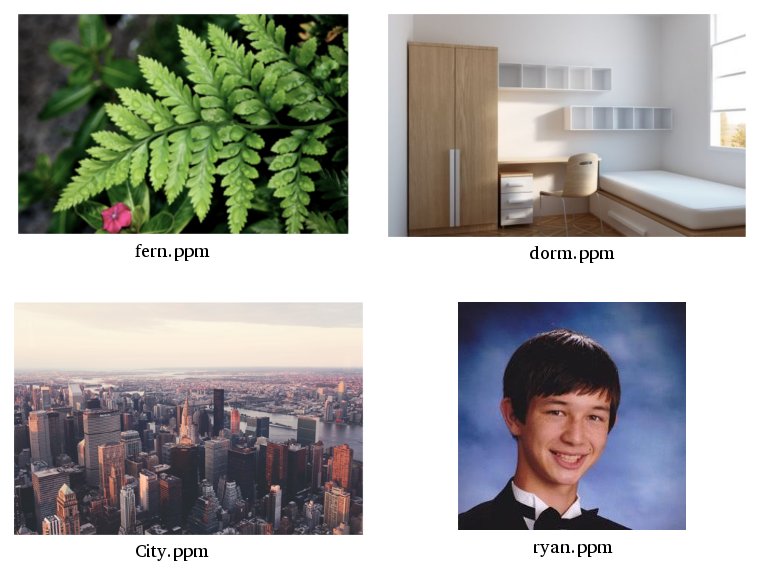
\includegraphics[scale=0.5]{images}\\
\textbf{Figure A1: } The images used during experimentation.\\ 
\end{center}

\vspace{1em}
\begin{center}
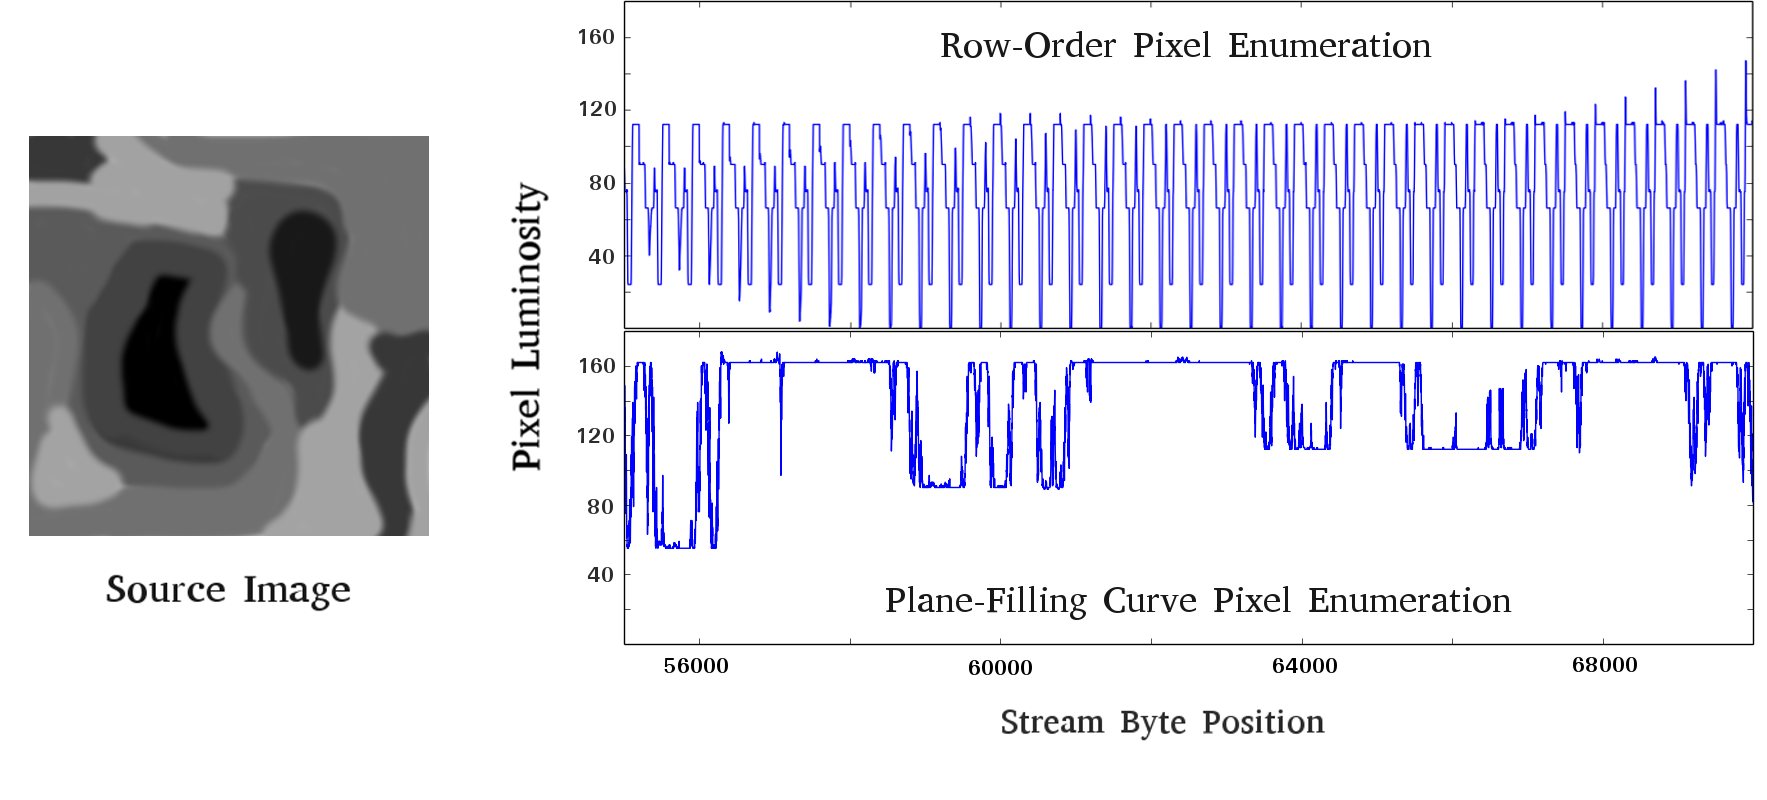
\includegraphics[scale=0.24]{srf_signal}\\
\textbf{Figure A2: } A comparison of the signal produced by row-order vs. plane-filling curve pixel enumeration.\\ 
\end{center}

\vspace{1em}
\begin{center}
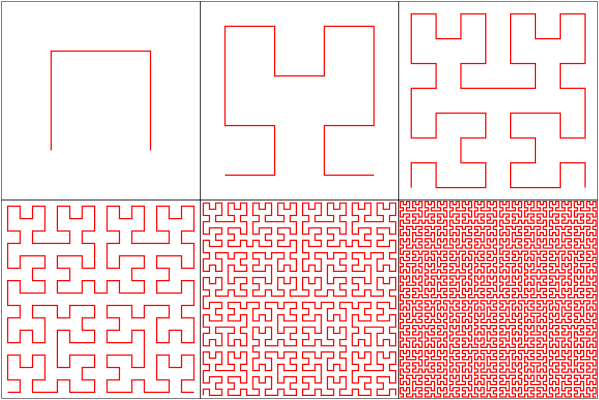
\includegraphics[scale=0.55]{hilbert_curve}\\
\textbf{Figure A3: } Approximations of the Hilbert Plane filling curve.
\end{center}

\end{document}
